\section{Input Data definition for Classical and Event Based PSHA, Disaggregation and UHS}
Input data for probabilistic based seismic hazard analysis (Classical, Event based, Disaggregation, and UHS) are structured in terms of a:
\begin{itemize}
\item file describing the Seismic Source System, that is the set of initial source models and associated epistemic uncertainties needed to model the seismic activity in the region of interest.
\item file describing the Ground Motion System, that is the set of ground motion prediction equations, per tectonic region type, needed to model the ground motion shaking in the region of interest.
\end{itemize}
The paths to the Seismic Source and Ground Motion System files are given in the 
\Verb+SOURCE_MODEL_LOGIC_TREE_FILE+ and \Verb
+GMPE_LOGIC_TREE_FILE+ keys, respectively, both defined in the \Verb+[HAZARD]+ section of the configuration file:\\
\begin{Verbatim}[frame=single, commandchars=\\\{\}, samepage=true]
[\textcolor{red}{HAZARD}]
...
SOURCE_MODEL_LOGIC_TREE_FILE=/PATH/TO/SEISMIC/SOURCE/SYSTEM/FILE
GMPE_LOGIC_TREE_FILE=/PATH/TO/GROUND/MOTION/SYSTEM/FILE
...
\end{Verbatim}
Both files are in NRML format and the information content is organized in a logic tree structure. Section \ref{ltd} provides a general
description about logic tree definition in NRML while sections \ref{sss} and \ref{gms} explain how the NRML logic tree structure is 
utilized for the seismic source and ground motion system definitions, respectively.

\subsection{Logic Tree definition in NRML}\label{ltd}
In the NRML schema, a logic tree is defined in terms of three main objects:
\begin{itemize}
\item branching level
\item branch set
\item individual branch
\end{itemize}
A schematic representation of these three objects is provided in Figure \ref{glts}. A branching level identifies the position in a tree where branching occurs while a branch set identifies a collection of branches (i.e. individual branches) whose weights sum to 1.\\
\begin{figure}[!htbp]
\begin{center}
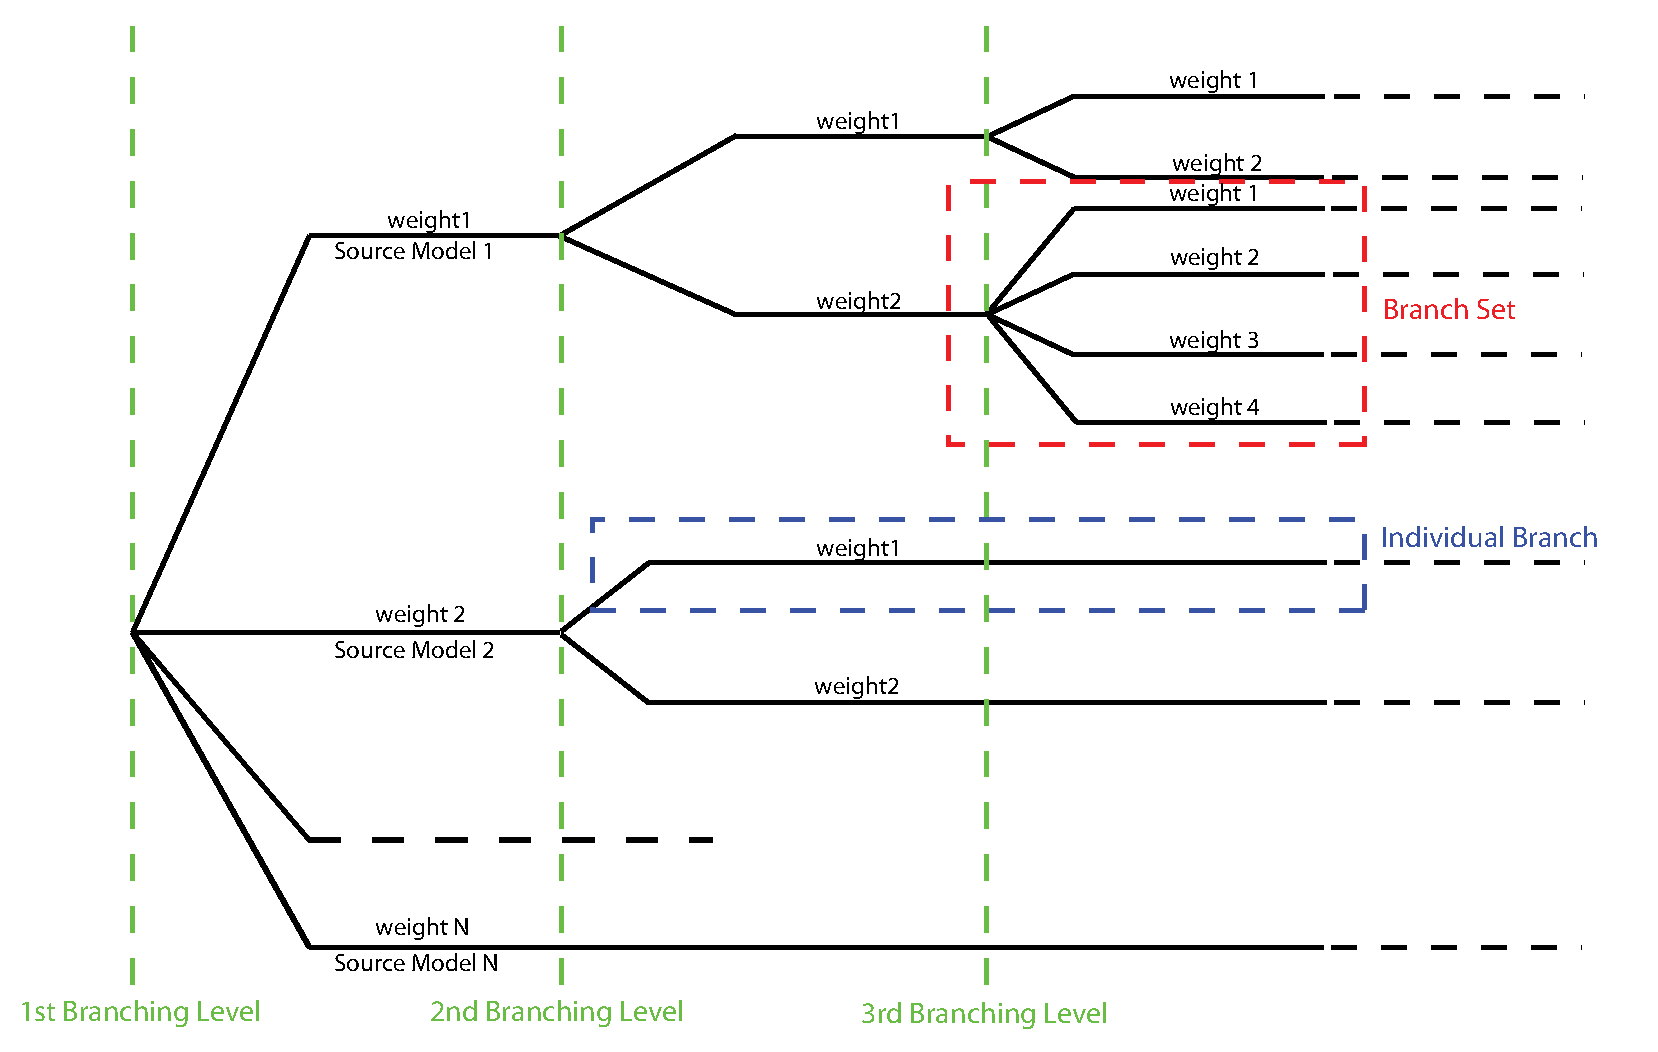
\includegraphics[width=15cm]{./oqum_Figures/GenericLogicTreeStructure.eps}
\caption{Generic Logic Tree structure as described in terms of branching levels, branch sets, and individual branches.}
\label{glts}
\end{center}
\end{figure}
In the NRML schema, a logic tree structure is defined through the a \Verb+logicTree+ element: 
\begin{Verbatim}[frame=single, commandchars=\\\{\}, samepage=true]
<\textcolor{red}{logicTree} logicTreeID="ID">
...
</\textcolor{red}{logicTree}>
\end{Verbatim}
A \Verb+logicTree+ is defined as a sequence of \Verb+logicTreeBranchingLevel+ elements. The position in the sequence specifies in which level of the tree the branching level is located. That is, the first logicTreeBranchingLevel element in the sequence represents the first level in the tree, the second element the second level in the tree, and so on.
\begin{Verbatim}[frame=single, commandchars=\\\{\}, samepage=true]
<\textcolor{red}{logicTree} logicTreeID="ID">
	<\textcolor{green}{logicTreeBranchingLevel} branchingLevelID="ID_1">
		...
	</\textcolor{green}{logicTreeBranchingLevel}>
	<\textcolor{green}{logicTreeBranchingLevel} branchingLevelID="ID_2">
		...
	</\textcolor{green}{logicTreeBranchingLevel}>
	....
	<\textcolor{green}{logicTreeBranchingLevel} branchingLevelID="ID_N">
		...
	</\textcolor{green}{logicTreeBranchingLevel}>
</\textcolor{red}{logicTree}>
\end{Verbatim}
No restrictions are present on the number of tree levels that can be defined.\\
A \Verb+logicTreeBranchingLevel+ is defined as a sequence of \Verb+logicTreeBranchSet+ elements. Each \Verb+logicTreeBranchSet+ defines a particular epistemic uncertainty inside a branching level. A branch set has two required attributes (\Verb+branchSetID+ and \Verb+uncertaintyType+ (defining the type of epistemic uncertainty the branch set is defining))
\begin{Verbatim}[frame=single, commandchars=\\\{\}, samepage=true]
<\textcolor{red}{logicTree} logicTreeID="ID">
...
	<\textcolor{green}{logicTreeBranchingLevel} branchingLevelID="ID_#">
		<\textcolor{blue}{logicTreeBranchSet} branchSetID="ID_1"
			uncertaintyType="UNCERTAINTY_TYPE">
			...
		</\textcolor{blue}{logicTreeBranchSet}>
		<\textcolor{blue}{logicTreeBranchSet} branchSetID="ID_2"
			uncertaintyType="UNCERTAINTY_TYPE">
			...
		</\textcolor{blue}{logicTreeBranchSet}>
		...
		<\textcolor{blue}{logicTreeBranchSet} branchSetID="ID_N"
			uncertaintyType="UNCERTAINTY_TYPE">
			...
		</\textcolor{blue}{logicTreeBranchSet}>
	</\textcolor{green}{logicTreeBranchingLevel}>
...
</\textcolor{red}{logicTree}>
\end{Verbatim}
Possible values for the \Verb+uncertaintyType+ attribute are:
\begin{itemize}
\item \Verb+gmpeModel+: identifying epistemic uncertainties on ground motion prediction equations
\item \Verb+sourceModel+: identifying epistemic uncertainties on source models
\item \Verb+maxMagGRRelative+: identifying epistemic uncertainties (relative: that is increments) to be added (or subtracted, depending on the sign of the increment) to the Gutenberg-Richter maximum magnitude value.
\item \Verb+bGRRelative+: identifying epistemic uncertainties (relative) to be applied to the Gutenberg-Richter b value.
\item \Verb+abGRAbsolute+:identifying epistemic uncertainties (absolute: that is new values used to replace original values) on the Gutenberg-Richter a and b values.
\item \Verb+maxMagGRAbsolute+: identifying epistemic uncertainties (absolute) on the Gutenberg-Richter maximum magnitude.
\end{itemize}
No restrictions are given on the number of branch sets that can be defined inside a branching level.\\
A \Verb+branchSet+ is defined as a sequence of  \Verb+logicTreeBranch+ elements, each defined by an \Verb+uncertaintyModel+ element (a string identifying an uncertainty model; the content of the string varies with the uncertaintyType attribute value of the branchSet element) and the uncertaintyWeight element (specifying the probability/weight associated to the uncertaintyModel):
\begin{Verbatim}[frame=single, commandchars=\\\{\}, samepage=true]
<\textcolor{red}{logicTree} logicTreeID="ID">
...
	<\textcolor{green}{logicTreeBranchingLevel} branchingLevelID="ID_#">
		...
		<\textcolor{blue}{logicTreeBranchSet} branchSetID="ID_#"
				uncertaintyType="UNCERTAINTY_TYPE">
			<\textcolor{magenta}{logicTreeBranch} branchID="ID_1">
				<uncertaintyModel>
				UNCERTAINTY_MODEL
				</uncertaintyModel>
				<uncertaintyWeight>
				UNCERTAINTY_WEIGHT
				</uncertaintyWeight>
			</\textcolor{magenta}{logicTreeBranch}>
			...
			<\textcolor{magenta}{logicTreeBranch} branchID="ID_N">
				<uncertaintyModel>
				UNCERTAINTY_MODEL
				</uncertaintyModel>
				<uncertaintyWeight>
				UNCERTAINTY_WEIGHT
				</uncertaintyWeight>
			</\textcolor{magenta}{logicTreeBranch}>
		</\textcolor{blue}{logicTreeBranchSet}>
		...
	</\textcolor{green}{logicTreeBranchingLevel}>
...
</\textcolor{red}{logicTree}>
\end{Verbatim}
Depending on the \Verb+uncertaintyType+ the content of the \Verb+<uncertaintyModel>+ element changes:
\begin{itemize}
\item if \Verb+uncertaintyType="gmpeModel"+, the uncertainty model contains the name of a ground motion prediction equation (a list of available GMPEs are given in appendix A), e.g.:
\begin{Verbatim}[frame=single, commandchars=\\\{\}, samepage=true]
<uncertaintyModel>GMPE_NAME</uncertaintyModel>
\end{Verbatim}
\item if \Verb+uncertaintyType="sourceModel"+, the uncertainty model contains the paths to a source model file, e.g.:
\begin{Verbatim}[frame=single, commandchars=\\\{\}, samepage=true]
<uncertaintyModel>SOURCE_MODEL_FILE_PATH</uncertaintyModel>
\end{Verbatim}
\item if \Verb+uncertaintyType="maxMagGRRelative"+, the uncertainty model contains the increment to be added (or subtracted, depending on the sign) to the Gutenberg-Richter maximum magnitude:
\begin{Verbatim}[frame=single, commandchars=\\\{\}, samepage=true]
<uncertaintyModel>MAX_MAGNITUDE_INCREMENT</uncertaintyModel>
\end{Verbatim}
\item if \Verb+uncertaintyType="bGRRelative"+, the uncertainty model contains the increment to be added (or subtracted, depending on the sign) to the Gutenberg-Richter b value:
\begin{Verbatim}[frame=single, commandchars=\\\{\}, samepage=true]
<uncertaintyModel>B_VALUE_INCREMENT</uncertaintyModel>
\end{Verbatim}
\item if \Verb+uncertaintyType="abGRAbsolute"+, the uncertainty model contains one (if the uncertainty apply to a source with only one Gutenberg-Richter magnitude frequency distribution) or more (if the source has more than one magnitude frequency distributions) a and b pairs:
\begin{Verbatim}[frame=single, commandchars=\\\{\}, samepage=true]
<uncertaintyModel>
A_VALUE_1 B_VALUE_1
 ... 
A_VALUE_N B_VALUE_N
</uncertaintyModel>
\end{Verbatim}
\item if \Verb+uncertaintyType="maxMagGRAbsolute"+, the uncertainty model contains one or more (depending on the number of magnitude frequency distributions in the source) Gutenberg-Richter maximum magnitude values:
\begin{Verbatim}[frame=single, commandchars=\\\{\}, samepage=true]
<uncertaintyModel>
MAX_MAGNITUDE_1
 ... 
MAX_MAGNITUDE_N
</uncertaintyModel>
\end{Verbatim}
\end{itemize}
No restrictions are given on the number of \Verb+logicTreeBranch+ elements that can be defined in a \Verb+logicTreeBranchSet+, as long as the uncertainty weights sum to 1.0.\\
The \Verb+logicTreeBranchSet+ element offers also a number of optional attributes allowing for complex tree definitions:
\begin{itemize}
\item \Verb+applyToBranches+: specifies to which \Verb+logicTreeBranch+ elements (one or more), in the previous branching level, the branch set is linked to. The linking is established by defining the IDs of the branches to link to:
\begin{Verbatim}[frame=single, commandchars=\\\{\}, samepage=true]
applyToBranches="branchID1 branchID2 .... branchIDN"
\end{Verbatim}
The default is the keyword ALL, which means that a branch set is by default linked to all branches in the previous branching level. By specifying one or more branches to which the branch set links to, non-symmetric logic trees can be defined.
\item \Verb+applyToSources+: specifies to which source in a source model the uncertainty applies to. Sources are specified in terms of their IDs:
\begin{Verbatim}[frame=single, commandchars=\\\{\}, samepage=true]
applyToSources="srcID1 srcID2 .... srcIDN"
\end{Verbatim}
\item \Verb+applyToSourceType+: specifies to which source type the uncertainty applies to.
Only one source typology can be defined (\Verb+area+, \Verb+point+, \Verb+simpleFault+, \Verb+complexFault+), e.g.:
\begin{Verbatim}[frame=single, commandchars=\\\{\}, samepage=true]
applyToSources="area"
\end{Verbatim}
\item \Verb+applyToTectonicRegionType+: specifies to which tectonic region type the uncertainty applies to. Only one tectonic region type can be defined (\Verb+Active Shallow Crust+, \Verb+Stable Shallow Crust+,  \Verb+Subduction Interface+, \Verb+Subduction IntraSlab+, \Verb+Volcanic+), e.g.:
\begin{Verbatim}[frame=single, commandchars=\\\{\}, samepage=true]
applyToTectonicRegionType="Active Shallow Crust"
\end{Verbatim}
\end{itemize}

\subsection{The Seismic Source System definition}\label{sss}
The Seismic Source System is defined in a \Verb+logicTreeElement+ with the following constrains:
\begin{itemize}
\item The first branching level can contain only one branch set. This branch set must define uncertainties in the source model (that is \Verb+uncertaintyType="sourceModel"+)
\item Subsequent branching levels can define uncertainties of type: \Verb+maxMagGRRelative+, \Verb+bGRRelative+, \Verb+abGRAbsolute+, \Verb+maxMagGRAbsolute+. Relative uncertainties are applied assuming conservation of total moment rate.
\item In all branching levels but the first, only one optional attribute (\Verb+applyToSources+, \Verb+applyToSourceType+, \Verb+applyToTectonicRegionType+) can be defined. The first branching level does not accept any optional attribute.
\item If in a branching level, a branch set has \Verb+applyToBranches="ALL"+, then this branch set must be unique in the branching level. In other words, only one branch set with \Verb+applyToBranches="ALL"+ is allowed per branching level.
\item If in a branching level, more than one branch sets are defined, the attribute \Verb+applyToBranches+ must contain one or more branch IDs referring to branches that are only in the previous branching level and that are not already linked to other branch sets (in other words there cannot be two branch sets that link to the same branch).
\item In all branch sets, branch weights must sum to 1.
\end{itemize}
Figure \ref{lt1} shows an example of Seismic Source System consisting of two initial source models defined in the first branching level. In the second branching level, absolute uncertainties on Gutenberg-Richter a and b values are defined for source model 1 (\Verb+applyToBranches="_11"+). These uncertainties apply only to \Verb+area+ sources (applyToSourceType="area"). Same type of uncertainties are defined also for source model 2 (\Verb+applyToBranches="_12"+) but apply only to sources with IDs equal to \Verb+"_2"+ and \Verb+"_3"+ (\Verb+applyToSources="_2 _3"+). In the third branching level, absolute uncertainties on Gutenberg-Richter maximum magnitude are defined. These uncertainties apply to all source models in the previous branching level (the attribute \Verb+applyToBranches+ is absent, the default value \Verb+"ALL"+ is therefore assumed) but only to those sources that belongs to active shallow crust\\ (\Verb+applyToTectonicRegionType="Active Shallow Crust"+).
\begin{figure}[htbp]
\begin{center}
\begin{Verbatim}[frame=single, commandchars=\\\{\},fontsize=\scriptsize, samepage=true]
<\textcolor{red}{logicTree} logicTreeID="ID">
	<\textcolor{green}{logicTreeBranchingLevel} branchingLevelID="ID">
		<\textcolor{blue}{logicTreeBranchSet} branchSetID="ID"
		  uncertaintyType="\textcolor{orange}{sourceModel}">
			<\textcolor{magenta}{logicTreeBranch} branchID="_11">
			   <uncertaintyModel>SOURCE_MODEL_FILE_PATH</uncertaintyModel>
			   <uncertaintyWeight>WEIGHT</uncertaintyWeight>
			 </\textcolor{magenta}{logicTreeBranch}> 
			<\textcolor{magenta}{logicTreeBranch} branchID="_12">
			  <uncertaintyModel>SOURCE_MODEL_FILE_PATH</uncertaintyModel>
			  <uncertaintyWeight>WEIGHT</uncertaintyWeight>
			</\textcolor{magenta}{logicTreeBranch}>
		</\textcolor{blue}{logicTreeBranchSet}>
	</\textcolor{green}{logicTreeBranchingLevel}>
	<\textcolor{green}{logicTreeBranchingLevel} branchingLevelID="ID">
		<\textcolor{blue}{logicTreeBranchSet} branchSetID="ID" 
		    uncertaintyType="\textcolor{orange}{abGRAbsolute}"
		    applyToBranches="_11" 
		    applyToSourceType="area">
			<\textcolor{magenta}{logicTreeBranch} branchID="_11_12_21">
			   <uncertaintyModel>A_VALUE B_VALUE</uncertaintyModel>
			   <uncertaintyWeight>WEIGHT</uncertaintyWeight>
			</\textcolor{magenta}{logicTreeBranch}>
			<\textcolor{magenta}{logicTreeBranch} branchID="_11_12_22">
			   <uncertaintyModel>A_VALUE B_VALUE</uncertaintyModel>
			   <uncertaintyWeight>WEIGHT</uncertaintyWeight>
			</\textcolor{magenta}{logicTreeBranch}>  
		</\textcolor{blue}{logicTreeBranchSet}>
		<\textcolor{blue}{logicTreeBranchSet} branchSetID="ID" 
		   uncertaintyType="\textcolor{orange}{abGRAbsolute}"
	            applyToBranches="_12" 
		   applyToSources="_2 _3">
			<\textcolor{magenta}{logicTreeBranch} branchID="_13_21">
			   <uncertaintyModel>A_VALUE B_VALUE</uncertaintyModel>
			   <uncertaintyWeight>WEIGHT</uncertaintyWeight>
			   </\textcolor{magenta}{logicTreeBranch}>
			<\textcolor{magenta}{logicTreeBranch} branchID="_13_22">
			   <uncertaintyModel>A_VALUE B_VALUE</uncertaintyModel>
			   <uncertaintyWeight>WEIGHT</uncertaintyWeight>
			</\textcolor{magenta}{logicTreeBranch}>
		</\textcolor{blue}{logicTreeBranchSet}>
	</\textcolor{green}{logicTreeBranchingLevel}>
	<\textcolor{green}{logicTreeBranchingLevel} branchingLevelID="ID">
		<\textcolor{blue}{logicTreeBranchSet} branchSetID="ID" 
		   uncertaintyType="\textcolor{orange}{maxMagGRAbsolute}" 
		   applyToTectonicRegionType="Active Shallow Crust">
			<\textcolor{magenta}{logicTreeBranch} branchID="_31">
			   <uncertaintyModel>MAXIMUM_MAGNITUDE</uncertaintyModel>
			   <uncertaintyWeight>WEIGHT</uncertaintyWeight>
			</\textcolor{magenta}{logicTreeBranch}>
			<\textcolor{magenta}{logicTreeBranch} branchID="_32">
			   <uncertaintyModel>MAXIMUM_MAGNITUDE</uncertaintyModel>
			   <uncertaintyWeight>WEIGHT</uncertaintyWeight>
			</\textcolor{magenta}{logicTreeBranch}>
		</\textcolor{blue}{logicTreeBranchSet}>
	</\textcolor{green}{logicTreeBranchingLevel}>
</\textcolor{red}{logicTree}>
\end{Verbatim}
\caption{Example of Seismic Source System definition. Two source models are considered, and epistemic uncertainties (absolute) on Gutenberg-Richter a and b, and maximum magnitude are defined.}
\label{lt1}
\end{center}
\end{figure}

\subsection{The Ground Motion System definition}\label{gms}
The Ground Motion System is defined in a \Verb+logicTree+ element with the following constrains:
\begin{itemize}
\item Only one branch set can be defined per branching level.
\item Each branch set must define uncertainties of type \Verb+gmpeModel+.
\item All branch sets must define the applyToTectonicRegionType attribute. This is the only attribute allowed.
\item Each branch set must refer to a different tectonic region type.
\item In all branch sets, branch weights must sum to 1.
\end{itemize}
Figure \ref{lt2} shows an example of Ground Motion System as defined in a \Verb+logicTreeElement+. Each branching level contains only one \Verb+branchSet+, each referring to a different tectonic region type. Each branch set can contain a variable number of GMPEs.
\begin{figure}[htbp]
\begin{center}
\begin{Verbatim}[frame=single, commandchars=\\\{\},fontsize=\scriptsize, samepage=true]
<\textcolor{red}{logicTree} logicTreeID="ID">       
	<\textcolor{green}{logicTreeBranchingLevel} branchingLevelID="ID">
		<\textcolor{blue}{logicTreeBranchSet} branchSetID="ID" uncertaintyType="gmpeModel" 
		applyToTectonicRegionType="\textcolor{orange}{Active Shallow Crust}">
			<\textcolor{magenta}{logicTreeBranch} branchID="ID">
				<uncertaintyModel>GMPE_NAME</uncertaintyModel>
				<uncertaintyWeight>WEIGHT</uncertaintyWeight>
			</\textcolor{magenta}{logicTreeBranch}>
			<\textcolor{magenta}{logicTreeBranch} branchID="ID">
				<uncertaintyModel>GMPE_NAME</uncertaintyModel>
				<uncertaintyWeight>WEIGHT</uncertaintyWeight>
			</\textcolor{magenta}{logicTreeBranch}>                
		</\textcolor{blue}{logicTreeBranchSet}>       
	</\textcolor{green}{logicTreeBranchingLevel}>
		<\textcolor{green}{logicTreeBranchingLevel} branchingLevelID="ID">
		<\textcolor{blue}{logicTreeBranchSet} branchSetID="ID" uncertaintyType="gmpeModel" 
		applyToTectonicRegionType="\textcolor{orange}{Stable Shallow Crust}">
			<\textcolor{magenta}{logicTreeBranch} branchID="ID">
				<uncertaintyModel>GMPE_NAME</uncertaintyModel>
				<uncertaintyWeight>WEIGHT</uncertaintyWeight>
			</\textcolor{magenta}{logicTreeBranch}>
			<\textcolor{magenta}{logicTreeBranch} branchID="ID">
				<uncertaintyModel>GMPE_NAME</uncertaintyModel>
				<uncertaintyWeight>WEIGHT</uncertaintyWeight>
			</\textcolor{magenta}{logicTreeBranch}>                
		</\textcolor{blue}{logicTreeBranchSet}>       
	</\textcolor{green}{logicTreeBranchingLevel}>
		<\textcolor{green}{logicTreeBranchingLevel} branchingLevelID="ID">
		<\textcolor{blue}{logicTreeBranchSet} branchSetID="ID" uncertaintyType="gmpeModel" 
		applyToTectonicRegionType="\textcolor{orange}{Subduction IntraSlab}">
			<\textcolor{magenta}{logicTreeBranch} branchID="ID">
				<uncertaintyModel>GMPE_NAME</uncertaintyModel>
				<uncertaintyWeight>WEIGHT</uncertaintyWeight>
			</\textcolor{magenta}{logicTreeBranch}>
			<\textcolor{magenta}{logicTreeBranch} branchID="ID">
				<uncertaintyModel>GMPE_NAME</uncertaintyModel>
				<uncertaintyWeight>WEIGHT</uncertaintyWeight>
			</\textcolor{magenta}{logicTreeBranch}>                
		</\textcolor{blue}{logicTreeBranchSet}>       
	</\textcolor{green}{logicTreeBranchingLevel}>
	<\textcolor{green}{logicTreeBranchingLevel} branchingLevelID="ID">
		<\textcolor{blue}{logicTreeBranchSet} branchSetID="ID" uncertaintyType="gmpeModel" 
		applyToTectonicRegionType="\textcolor{orange}{Subduction Interface}">
			<\textcolor{magenta}{logicTreeBranch} branchID="ID">
				<uncertaintyModel>GMPE_NAME</uncertaintyModel>
				<uncertaintyWeight>WEIGHT</uncertaintyWeight>
			</\textcolor{magenta}{logicTreeBranch}>                
		</\textcolor{blue}{logicTreeBranchSet}>
	</\textcolor{green}{logicTreeBranchingLevel}>
	<\textcolor{green}{logicTreeBranchingLevel} branchingLevelID="ID">
		<\textcolor{blue}{logicTreeBranchSet} branchSetID="ID" uncertaintyType="gmpeModel" 
		applyToTectonicRegionType="\textcolor{orange}{Volcanic}">
			<\textcolor{magenta}{logicTreeBranch} branchID="ID">
				<uncertaintyModel>GMPE_NAME</uncertaintyModel>
				<uncertaintyWeight>WEIGHT</uncertaintyWeight>
			</\textcolor{magenta}{logicTreeBranch}>                
		</\textcolor{blue}{logicTreeBranchSet}>
	</\textcolor{green}{logicTreeBranchingLevel}>           
</\textcolor{red}{logicTree}>
\end{Verbatim}
\caption{Example of Ground Motion System definition. GMPEs are defined for the tectonic region types currently supported by OpenQuake.}
\label{lt2}
\end{center}
\end{figure}

\subsection{The Seismic Source Model definition}\label{seismicSourceNrml}
To complete the Seismic Source System definition the required seismic source models must be defined. A Seismic Source Model is defined as a collection of seismic sources. Four source typologies can be currently defined:
\begin{itemize}
\item Area
\item Point
\item Simple Fault
\item Complex Fault
\end{itemize}
Each source typology is identified by a specific element name in the nrML format:
\begin{itemize}
\item \Verb+areaSource+ (for Area)
\item \Verb+pointSource+ (for Point)
\item \Verb+simpleFaultSource+ (for Simple Fault)
\item \Verb+complexFaultSource+ (for Complex Fault)
\end{itemize}
Regardless of the source typology three common attributes must be defined:
\begin{itemize}
\item ID
\item name
\item tectonic region type 
\end{itemize}
\begin{Verbatim}[frame=single, commandchars=\\\{\},fontsize=\normalsize, samepage=true]
<\textcolor{red}{sourceModel} gml:id="ID">
	...
	<\textcolor{green}{areaSource} gml:id="SOURCE_ID">
		<gml:name>SOURCE_NAME</gml:name>
		<tectonicRegion>TECT_REGION_TYPE</tectonicRegion>
		...
	</\textcolor{green}{areaSource}>
	...
	<\textcolor{green}{pointSource} gml:id="SOURCE_ID">
		<gml:name>SOURCE_NAME</gml:name>
		<tectonicRegion>TECT_REGION_TYPE</tectonicRegion>
		...
	</\textcolor{green}{pointSource}>
	...
	<\textcolor{green}{simpleFaultSource} gml:id="SOURCE_ID">
		<gml:name>SOURCE_NAME</gml:name>
		<tectonicRegion>TECT_REGION_TYPE</tectonicRegion>
		...
	</\textcolor{green}{simpleFaultSource}>
	...
	<\textcolor{green}{complexFaultSource} gml:id="SOURCE_ID">
		<gml:name>SOURCE_NAME</gml:name>
		<tectonicRegion>TECT_REGION_TYPE</tectonicRegion>
		...
	</\textcolor{green}{complexFaultSource}>
	...
</\textcolor{red}{sourceModel}>
\end{Verbatim}
A single source model can therefore contain sources of different typologies, and no constrains are given on the number of sources that can be defined in a source model.

\subsubsection{Area source definition}
An area source can be utilized to describe a polygonal geographical region where seismicity is assumed to be uniform. The area source-specific elements are:
\begin{itemize}
\item \Verb+areaBoundary+: defines the area boundary.
\item \Verb+ruptureRateModel+: defines a MFD-Focal Mechanism pair.
\item \Verb+ruptureDepthDistribution+: defines the (top of) rupture depth distribution versus magnitude.
\item \Verb+hypocentralDepth+: defines ruptures' hypocentral depth.
\end{itemize}
More then one \Verb+ruptureRateModels+ can be defined in a single area source (giving the possibility to define specific MFDs for specific focal mechanisms).
\begin{Verbatim}[frame=single, commandchars=\\\{\},fontsize=\normalsize, samepage=true]
<\textcolor{red}{areaSource} gml:id="ID">
	<gml:name>NAME</gml:name>
	<tectonicRegion>TECT_REG_TYPE</tectonicRegion>
	<\textcolor{green}{areaBoundary}>
		...
	</\textcolor{green}{areaBoundary}>
	<\textcolor{blue}{ruptureRateModel}>
		...
	</\textcolor{blue}{ruptureRateModel}>
	<\textcolor{blue}{ruptureRateModel}>
		...
	</\textcolor{blue}{ruptureRateModel}>
	...
	...
	<\textcolor{blue}{ruptureRateModel}>
		...
	</\textcolor{blue}{ruptureRateModel}>
	<\textcolor{magenta}{ruptureDepthDistribution}>
		...
	</\textcolor{magenta}{ruptureDepthDistribution}>
	<\textcolor{orange}{hypocentralDepth}>
		...	
	</\textcolor{orange}{hypocentralDepth}>
</\textcolor{red}{areaSource}>
\end{Verbatim}
The area boundary is defined by a list of vertices coordinates (longitude, latitude) in a \Verb+LinearRing+ element defining the exterior boundary of a \Verb+Polygon+ element:
\begin{Verbatim}[frame=single, commandchars=\\\{\},fontsize=\normalsize, samepage=true]
<\textcolor{red}{areaBoundary}>
	<gml:\textcolor{green}{Polygon}>
		<gml:\textcolor{blue}{exterior}>
			<gml:\textcolor{magenta}{LinearRing}>
				<gml:\textcolor{orange}{posList}>
					LON_1 LAT_1
					LON_2 LAT_2
						...			
					LON_N LAT_N
				</gml:\textcolor{orange}{posList}>
			</gml:\textcolor{magenta}{LinearRing}>
		</gml:\textcolor{blue}{exterior}>
	</gml:\textcolor{green}{Polygon}>
</\textcolor{red}{areaBoundary}>
Polygon coordinates can be given in clock or counter-clock wise order.
\end{Verbatim}
The \Verb+ruptureRateModel+ element contains the definition of a magnitude frequency distribution (\Verb+truncatedGutenbergRichter+ or \Verb+evenlyDiscretizedIncrementalMFD+) and a focal mechanism (\Verb+focalMechanism+). That is:
\begin{Verbatim}[frame=single, commandchars=\\\{\},fontsize=\normalsize, samepage=true]
<\textcolor{red}{ruptureRateModel}>
	<\textcolor{green}{truncatedGutenbergRichter}>
		...
	</\textcolor{green}{truncatedGutenbergRichter}>
	<\textcolor{blue}{focalMechanism}>
		...
	</\textcolor{blue}{focalMechanism}>
</\textcolor{red}{ruptureRateModel}>
\end{Verbatim}
or:
\begin{Verbatim}[frame=single, commandchars=\\\{\},fontsize=\normalsize, samepage=true]
<\textcolor{red}{ruptureRateModel}>
	<\textcolor{green}{evenlyDiscretizedIncrementalMFD}>
		...
	</\textcolor{green}{evenlyDiscretizedIncrementalMFD}>
	<\textcolor{blue}{focalMechanism}>
		...
	</\textcolor{blue}{focalMechanism}>
</\textcolor{red}{ruptureRateModel}>
\end{Verbatim}
A truncated Gutenberg-Richter magnitude frequency distribution is defined in terms of minimum and maximum magnitudes, cumulative a value, and b value:
\begin{Verbatim}[frame=single, commandchars=\\\{\},fontsize=\normalsize, samepage=true]
<\textcolor{red}{truncatedGutenbergRichter}>
	<\textcolor{green}{aValueCumulative}>CUMULATIVE_A_VALUE</\textcolor{green}{aValueCumulative}>
	<\textcolor{blue}{bValue}>B_VALUE</\textcolor{blue}{bValue}>
	<\textcolor{magenta}{minMagnitude}>MINIMUM_MAGNITUDE</\textcolor{magenta}{minMagnitude}>
	<\textcolor{orange}{maxMagnitude}>MAXIMUM_MAGNITUDE</\textcolor{orange}{maxMagnitude}>
</\textcolor{red}{truncatedGutenbergRichter}>
\end{Verbatim}
the \Verb+CUMULATIVE_A_VALUE+ is assumed to be defined with respect to magnitude equal to 0.\\
The incremental evenly-discretized magnitude frequency distribution is defined instead as:
\begin{Verbatim}[frame=single, commandchars=\\\{\},fontsize=\normalsize, samepage=true]
<\textcolor{red}{evenlyDiscretizedIncrementalMFD} 
        \textcolor{green}{binSize}="BIN_SIZE"
 	 \textcolor{blue}{minVal}="MINIMUM_VALUE">
              RATE_1
              RATE_2
              ...
              RATE_N
</\textcolor{red}{evenlyDiscretizedIncrementalMFD}>
\end{Verbatim}
where \Verb+BIN_SIZE+ represents the discretization interval of the magnitude-frequency distribution, and \Verb+MINIMUM_VALUE+ represents the minimum value in the distribution (interpreted as the middle-point value of the first bin in the distribution). \Verb+RATE_1+...\Verb+RATE_N+ represent annual rates of occurrence starting from the minimum magnitude (\Verb+minVal+) up to the maximum magnitude.\\
The focal mechanism is defined in terms of strike, dip and rake values:
\begin{Verbatim}[frame=single, commandchars=\\\{\},fontsize=\normalsize, samepage=true]
<\textcolor{red}{focalMechanism} publicID="ID">
	<qml:\textcolor{green}{nodalPlanes}>
		<qml:\textcolor{blue}{nodalPlane1}>
			<qml:\textcolor{magenta}{strike}>
			<qml:value>STRIKE_VALUE</qml:value>
			</qml:\textcolor{magenta}{strike}>
			<qml:\textcolor{orange}{dip}>
			<qml:value>DIP_VALUE</qml:value>
			</qml:\textcolor{orange}{dip}>
			<qml:\textcolor{violet}{rake}>
			<qml:value>RAKE_VALUE</qml:value>
			</qml:\textcolor{violet}{rake}>
		</qml:\textcolor{blue}{nodalPlane1}>
	</qml:\textcolor{green}{nodalPlanes}>
</\textcolor{red}{focalMechanism}>
 \end{Verbatim}
where
\begin{alltt} \(0\degree \leq\) STRIKE_VALUE \(\leq 360\degree\) \end{alltt}
\begin{alltt} \(0\degree \leq\) DIP_VALUE \(\leq 90\degree\) \end{alltt}
\begin{alltt} \(-180\degree \leq\) RAKE_VALUE \(\leq +180\degree\) \end{alltt}
The \Verb+ruptureDepthDistribution+ contains a list of magnitude and depth values:
\begin{Verbatim}[frame=single, commandchars=\\\{\},fontsize=\normalsize, samepage=true]
<\textcolor{red}{ruptureDepthDistribution}>
	<\textcolor{green}{magnitude}>MAG_1 MAG_2 ... MAG_N</\textcolor{green}{magnitude}>
	<\textcolor{blue}{depth}>DEPTH_1 DEPTH_2 ... DEPTH_N</\textcolor{blue}{depth}>
</\textcolor{red}{ruptureDepthDistribution}>
\end{Verbatim}
The magnitude values define the bin edges of the distribution, that is:
\begin{alltt}MAG_1 \(\leq\) m \(<\) MAG_2, top of rupture depth = DEPTH_1 \end{alltt}
\begin{alltt}MAG_2 \(\leq\) m \(<\) MAG_3, top of rupture depth = DEPTH_2 \end{alltt}
		...
\begin{alltt}MAG_N-1 \(\leq\) m \(<\) MAG_N, top of rupture depth = DEPTH_N-1 \end{alltt}
\begin{alltt}m \(\geq\) MAG_N, top of rupture depth = DEPTH_N \end{alltt}
The hypocentral depth is specified by a single value:
\begin{Verbatim}[frame=single, commandchars=\\\{\},fontsize=\normalsize, samepage=true]
<\textcolor{red}{hypocentralDepth}>HYPOCENTRAL_DEPTH</\textcolor{red}{hypocentralDepth}>
\end{Verbatim}

\subsubsection{Point source definition}
The point source definition follows the same schema of the area source definition, the only
difference being the absence of the \Verb+areaBoundary+ element, that is replaced by a
\Verb+location+ element defining the coordinates of a single geographic site:
\begin{Verbatim}[frame=single, commandchars=\\\{\},fontsize=\normalsize, samepage=true]
<\textcolor{red}{pointSource} gml:id="ID">
	<gml:name>NAME</gml:name>
	<tectonicRegion>TECT_REG_TYPE</tectonicRegion>
	<\textcolor{green}{location}>
		...
	</\textcolor{green}{location}>
	<\textcolor{blue}{ruptureRateModel}>
		...
	</\textcolor{blue}{ruptureRateModel}>
	<\textcolor{blue}{ruptureRateModel}>
		...
	</\textcolor{blue}{ruptureRateModel}>
	...
	...
	<\textcolor{blue}{ruptureRateModel}>
		...
	</\textcolor{blue}{ruptureRateModel}>
	<\textcolor{magenta}{ruptureDepthDistribution}>
		...
	</\textcolor{magenta}{ruptureDepthDistribution}>
	<\textcolor{orange}{hypocentralDepth}>
		...	
	</\textcolor{orange}{hypocentralDepth}>
</\textcolor{red}{pointSource}>
\end{Verbatim}
where the \Verb+location+ element is defined as follows:
\begin{Verbatim}[frame=single, commandchars=\\\{\},fontsize=\normalsize, samepage=true]
<\textcolor{red}{location}>
	<gml:\textcolor{green}{Point}>
	<gml:pos>LON LAT</gml:pos>
	</gml:\textcolor{green}{Point}>
</\textcolor{red}{location}>
\end{Verbatim}

\subsubsection{Simple fault source definition}
The fault source-specific elements are:
\begin{itemize}
\item \Verb+rake+: defines the rake value.
\item \Verb+truncatedGutenbergRichter+ or \Verb+evenlyDiscretizedIncrementalMFD+: define the magnitude frequency distribution.
\item \Verb+simpleFaultGeometry+: defines the fault surface geometry.
\end{itemize}
\begin{Verbatim}[frame=single, commandchars=\\\{\},fontsize=\normalsize, samepage=true]
<\textcolor{red}{simpleFaultSource} gml:id="ID">
	<gml:name>SOURCE_NAME</gml:name>
	<tectonicRegion>TECT_REG_TYPE</tectonicRegion>
	<\textcolor{green}{rake}>
	...
	</\textcolor{green}{rake}>
	<\textcolor{blue}{truncatedGutenbergRichter}>
	...
	</\textcolor{blue}{truncatedGutenbergRichter}>
		\textit{OR}
	<\textcolor{blue}{evenlyDiscretizedIncrementalMFD}>
	...
	</\textcolor{blue}{evenlyDiscretizedIncrementalMFD}>
	<\textcolor{magenta}{simpleFaultGeometry}>
	...
	</\textcolor{magenta}{simpleFaultGeometry}>
</\textcolor{red}{simpleFaultSource}>
\end{Verbatim}
The \Verb+rake+ element contains a single rake value:
\begin{Verbatim}[frame=single, commandchars=\\\{\},fontsize=\normalsize, samepage=true]
<\textcolor{red}{rake}>RAKE_VALUE</\textcolor{red}{rake}>
\end{Verbatim}
The \Verb+simpleFaultGeometry+ element is defined as follows:
\begin{Verbatim}[frame=single, commandchars=\\\{\},fontsize=\normalsize, samepage=true]
<\textcolor{red}{simpleFaultGeometry} gml:id="ID">
	<\textcolor{green}{faultTrace}>
		<gml:\textcolor{blue}{LineString}>
			<gml:posList>
				LON1 LAT1 DEPTH1
				LON2 LAT2 DEPTH2
				...
				LONN LATN DEPTHN
			</gml:posList>
		</gml:\textcolor{blue}{LineString}>
	</\textcolor{green}{faultTrace}>
	<\textcolor{magenta}{dip}>DIP_VALUE</\textcolor{magenta}{dip}>
	<\textcolor{orange}{upperSeismogenicDepth}>UPPER_DEPTH</\textcolor{orange}{upperSeismogenicDepth}>
	<\textcolor{violet}{lowerSeismogenicDepth}>LOWER_DEPTH</\textcolor{violet}{lowerSeismogenicDepth}>
</\textcolor{red}{simpleFaultGeometry}>
\end{Verbatim}
The fault trace is defined as a 3D line, each point in the line being defined by longitude, latitude, and depth values. Fault trace coordinates must be given in the (positive) strike direction, in this way the fault surface is correctly constructed, dipping down to the right of the strike direction. Dip is specified by a single value, as well as the upper and lower seismogenic depths. 

\subsubsection{Complex fault source definition}
The complex fault source definition follows closely the simple fault source definition, the only difference being the absence of the \Verb+simpleFaultGeometry+ element, that is replaced by a \Verb+complexFaultGeometry+ element.
\begin{Verbatim}[frame=single, commandchars=\\\{\},fontsize=\normalsize, samepage=true]
<\textcolor{red}{complexFaultSource} gml:id="ID">
	<gml:name>NAME</gml:name>
	<tectonicRegion>TECT_REG_TYPE</tectonicRegion>
	<\textcolor{green}{rake}>RAKE_VALUE</\textcolor{green}{rake}>
	<\textcolor{blue}{truncatedGutenbergRichter}>
	...
	</\textcolor{blue}{truncatedGutenbergRichter}>
		\textit{OR}
	<\textcolor{blue}{evenlyDiscretizedIncrementalMFD}>
	...
	</\textcolor{blue}{evenlyDiscretizedIncrementalMFD}>
	<\textcolor{magenta}{complexFaultGeometry}>
	...
	</\textcolor{magenta}{complexFaultGeometry}>
</\textcolor{red}{complexFaultSource}>
\end{Verbatim}
The geometry is specified by the fault's top and bottom edge coordinates (in the \Verb+faultTopEdge+ and \Verb+faultBottomEdge+ elements). Coordinates must be given in the (positive) strike direction, in this way the fault surface is correctly constructed, dipping down to the right of the strike direction.
\begin{Verbatim}[frame=single, commandchars=\\\{\},fontsize=\normalsize, samepage=true]
<\textcolor{red}{complexFaultGeometry}>
	<\textcolor{green}{faultEdges}>
		<\textcolor{blue}{faultTopEdge}>
			<gml:LineString>
				<gml:posList>
					LON1 LAT1 DEPTH1
					LON2 LAT2 DEPTH2
					..
					LONN LATN DEPTHN
				</gml:posList>
			</gml:LineString>
		</\textcolor{blue}{faultTopEdge}>
		<\textcolor{magenta}{faultBottomEdge}>
			<gml:LineString>
				<gml:posList>
					LON1 LAT1 DEPTH1
					LON2 LAT2 DEPTH2
					..
					LONN LATN DEPTHN
				</gml:posList>
			</gml:LineString>
		</\textcolor{magenta}{faultBottomEdge}>
	</\textcolor{green}{faultEdges}>
</\textcolor{red}{complexFaultGeometry}>
\end{Verbatim}

\section{Configuration Parameters for Classical and Event Based PSHA, Disaggregation and UHS}
Configuration parameters can be broadly divided into five main groups:
\begin{itemize}
\item Source Model parameters
\item GMPE parameters
\item Site parameters
\item Logic Tree parameters
\item Calculator specific parameters
\end{itemize}

\subsection{Source Model parameters}
Source Model parameters define how seismic sources are modeled by the engine in order to create the earthquake rupture forecast (ERF).\\
\subsubsection{Area source parameters}
Each source typology has its own set of parameters. For area sources, the following keys must be set:
\begin{itemize}
\item \Verb+INCLUDE_AREA_SOURCES+: if \Verb+true+ all area sources in the source model are included in the ERF calculation. They are exclude if \Verb+false+.
\item \Verb+TREAT_AREA_SOURCE_AS+: specifies how ruptures in area sources must be modeled. Allowed values are:
\begin{itemize}
\item \Verb+Point Sources+
\item \Verb+Line Sources (random or given strike)+
\item \Verb+Cross Hair Line Sources+
\item \Verb+16 Spoked Line Sources+
\end{itemize}
\item \Verb+AREA_SOURCE_DISCRETIZATION+: defines area source region discretization step (in decimal degrees).
\item \Verb+AREA_SOURCE_MAGNITUDE_SCALING_RELATIONSHIP+: specifies the magnitude scaling relationship used for modeling finite ruptures (list of available scaling relationships are given in Appendix B).
\end{itemize}

\subsubsection{Point source parameters}
Point sources require similar parameters:
\begin{itemize}
\item \Verb+INCLUDE_GRID_SOURCES+: if \Verb+true+ all point sources in the source model are included in the ERF calculation. They are exclude if \Verb+false+.
\item \Verb+TREAT_GRID_SOURCE_AS+: specifies how ruptures in point sources must be modeled. Allowed values are:
\begin{itemize}
\item \Verb+Point Sources+
\item \Verb+Line Sources (random or given strike)+
\item \Verb+Cross Hair Line Sources+
\item \Verb+16 Spoked Line Sources+
\end{itemize}
\item \Verb+GRID_SOURCE_MAGNITUDE_SCALING_RELATIONSHIP+: specifies the magnitude scaling relationship used for modeling finite ruptures (list of available scaling relationships are given in Appendix B).
\end{itemize}

\subsubsection{Simple Fault source parameters}
Simple fault sources require the following parameters:
\begin{itemize}
\item \Verb+INCLUDE_FAULT_SOURCE+: if \Verb+true+ all simple fault sources in the source model are included in the ERF calculation. They are exclude if \Verb+false+.
\item \Verb+FAULT_RUPTURE_OFFSET+: specifies the amount by which ruptures are offset on the fault (in km)
\item \Verb+FAULT_SURFACE_DISCRETIZATION+: specifies the fault surface discretization step (in km).
\item \Verb+FAULT_MAGNITUDE_SCALING_RELATIONSHIP+: specifies the magnitude scaling relationship used for modeling finite ruptures (list of available scaling relationships are given in Appendix B).
\item \Verb+FAULT_MAGNITUDE_SCALING_SIGMA+: the standard deviation of log(Length) or log(Area)
\item \Verb+RUPTURE_ASPECT_RATIO+: rupture aspect ratio (rupture length / rupture width)
\item \Verb+RUPTURE_FLOATING_TYPE+: rupture floating algorithm. Allowed values are:
\begin{itemize}
\item \Verb+Only along strike ( rupture full DDW)+
\item \Verb+Along strike and down dip+
\item \Verb+Along strike & centered down dip+
\end{itemize}
\end{itemize}

\subsubsection{Complex Fault source parameters}
Complex fault sources require the same set of parameters:
\begin{itemize}
\item \Verb+INCLUDE_SUBDUCTION_FAULT_SOURCE+: if \Verb+true+ all complex fault sources in the source model are included in the ERF calculation. They are exclude if \Verb+false+.
\item \Verb+SUBDUCTION_FAULT_RUPTURE_OFFSET+: specifies the amount by which ruptures are offset on the fault (in km)
\item \Verb+SUBDUCTION_FAULT_SURFACE_DISCRETIZATION+: specifies the fault surface discretization step (in km).
\item \Verb+SUBDUCTION_FAULT_MAGNITUDE_SCALING_RELATIONSHIP+: specifies the magnitude scaling relationship used for modeling finite ruptures (list of available scaling relationships are given in Appendix B).
\item \Verb+SUBDUCTION_FAULT_MAGNITUDE_SCALING_SIGMA+: the standard deviation of log(Length) or log(Area)
\item \Verb+SUBDUCTION_RUPTURE_ASPECT_RATIO+: rupture aspect ratio (rupture length / rupture width)
\item \Verb+SUBDUCTION_RUPTURE_FLOATING_TYPE+: rupture floating algorithm. Allowed values are:
\begin{itemize}
\item \Verb+Only along strike ( rupture full DDW)+
\item \Verb+Along strike and down dip+
\item \Verb+Along strike & centered down dip+
\end{itemize}
\end{itemize}

\subsection{GMPE parameters}
The GMPE parameters configures the GMPEs chosen for calculation. The currently supported parameters are:
\begin{itemize}
\item \Verb+COMPONENT+: specifies the GMPE component. Allowed values are:
\begin{itemize}
\item \Verb+Average Horizontal+
\item \Verb+Average Horizontal (GMRotI50)+
\item \Verb+Random Horizontal+
\item \Verb+Greater of Two Horz.+
\item \Verb+Vertical+
\end{itemize}
\item \Verb+INTENSITY_MEASURE_TYPE+: Allowed options are:
\begin{itemize}
\item \Verb+PGA+: (g)
\item \Verb+PGD+: (cm)
\item \Verb+PGV+: (cm/s)
\item \Verb+SA+: (g)
\end{itemize}
\item \Verb+PERIOD+: spectral acceleration period (in seconds)
\item \Verb+DAMPING+: in percent
\item \Verb+GMPE_TRUNCATION_TYPE+: truncation algorithm for the GMPE distribution. Allowed values are:
\begin{itemize}
\item \Verb+None+: no truncation is applied.
\item \Verb+1 Sided+: truncation of upper side of distribution only.
\item \Verb+2 Sided+: truncation of both upper and lower sides of distribution.
\end{itemize}
\item \Verb+TRUNCATION_LEVEL+: units of sigma for GMPE distribution truncation.
\item \Verb+STANDARD_DEVIATION_TYPE+: type of standard deviation in the GMPE distribution. Allowed values are:
\begin{itemize}
\item \Verb+Total+
\item \Verb+Inter-Event+
\item \Verb+Intra-Event+
\item \Verb+None (zero)+
\end{itemize}
\end{itemize}

\subsection{Site parameters}
Site parameters describe site conditions that are used by GMPEs:
\begin{itemize}
\item \Verb+REFERENCE_VS30_VALUE+: shear wave velocity in the uppermost 30 meters (in m/s)
\item \Verb+VS30_TYPE+: allowed values:
\begin{itemize}
\item \Verb+measured+
\item \Verb+inferred+
\end{itemize}
\item \Verb+DEPTHTO1PT0KMPERSEC+: depth to where shear-wave velocity is equal to 1.0 km/s (in m).
\item \Verb+REFERENCE_DEPTH_TO_2PT5KM_PER_SEC_PARAM+: depth to where shear-wave velocity is equal to 2.5 km/s (in km).
\end{itemize}

\subsection{Logic Tree parameters}
Logic tree parameters configure the logic tree processing:
\begin{itemize}
\item \Verb+NUMBER_OF_LOGIC_TREE_SAMPLES+: number of logic tree traversals (obtained through random sampling of tree branches).
\item \Verb+SOURCE_MODEL_LT_RANDOM_SEED+: seed number for random number generator used for sampling the source model logic tree.
\item \Verb+GMPE_LT_RANDOM_SEED+: seed number for random number generator used for sampling the GMPE logic tree.
\end{itemize}

\subsection{Classical PSHA parameters}
Parameters required for configuring the Classical PSHA calculator are:
\begin{itemize}
\item \Verb+MINIMUM_MAGNITUDE+: minimum (moment) magnitude to be used in the ERF construction.
\item \Verb+INVESTIGATION_TIME+: time span (in years) for computing probability of exceedance.
\item \Verb+MAXIMUM_DISTANCE+: maximum distance of sources to be considered in the calculation. Sources more than this distance away are ignored.
\item \Verb+WIDTH_OF_MFD_BIN+: discretization interval for  magnitude-frequency distribution.
\item \Verb+INTENSITY_MEASURE_LEVELS+: comma separated list of intensity measure levels for which to compute probability of exceedance.
\item \Verb+COMPUTE_MEAN_HAZARD_CURVE+: if true, mean hazard curves are calculated and saved to file.
\item \Verb+POES+: on or more probability values for computing hazard maps (from mean hazard curves).
\item \Verb+QUANTILE_LEVELS+: one or more quantile levels for computing quantile hazard curves.
\end{itemize}

\subsection{Event Based PSHA parameters}
Parameters required for configuring the Event Based PSHA calculator are:
\begin{itemize}
\item \Verb+MINIMUM_MAGNITUDE+: minimum (moment) magnitude to be used in the ERF construction.
\item \Verb+INVESTIGATION_TIME+: time span (in years) for simulating stochastic event set.
\item \Verb+MAXIMUM_DISTANCE+: maximum distance of sources to be considered in the calculation. Sources more than this distance away are ignored.
\item \Verb+WIDTH_OF_MFD_BIN+: discretization interval for  magnitude-frequency distribution.
\item \Verb+NUMBER_OF_SEISMICITY_HISTORIES+: for each logic tree sample, the number of stochastic event sets to be generated.
\item \Verb+GMF_RANDOM_SEED+: seed number for random number generator used for ground motion field calculation.
\item \Verb+GROUND_MOTION_CORRELATION+: if true ground motion correlation is taken into account.
\item \Verb+GMF_OUTPUT+: if true, ground motion fields are saved to file.
\end{itemize}

\subsection{Disaggregation parameters}
Parameters required for configuring the Disaggregation calculator are:
\begin{itemize}
\item \Verb+MINIMUM_MAGNITUDE+: minimum (moment) magnitude to be used in the ERF construction.
\item \Verb+INVESTIGATION_TIME+: time span (in years) for computing probability of exceedance.
\item \Verb+MAXIMUM_DISTANCE+: maximum distance of sources to be considered in the calculation. Sources more than this distance away are ignored.
\item \Verb+WIDTH_OF_MFD_BIN+: discretization interval for  magnitude-frequency distribution.
\item \Verb+INTENSITY_MEASURE_LEVELS+: comma separated list of intensity measure levels for which to compute probability of exceedance.
\item \Verb+POES+: on or more probability values for computing disaggregation matrices.
\item \Verb+LATITUDE_BIN_LIMITS+: comma separated list of latitude values, defining latitude bin edges.
\item \Verb+LONGITUDE_BIN_LIMITS+: comma separated list of longitude values, defining longitude bin edges.
\item \Verb+MAGNITUDE_BIN_LIMITS+: comma separated list of magnitude values, defining magnitude bin edges.
\item \Verb+EPSILON_BIN_LIMITS+: comma separated list of epsilon values, defining epsilon bin edges.
\item \Verb+DISTANCE_BIN_LIMITS+: comma separated list of distance values, defining distance bin edges.
\item \Verb+DISAGGREGATION_RESULTS+: comma separated list of disaggregation type results. Allowed values:
\begin{itemize}
\item \Verb+MagPMF+: magnitude probability mass function (PMF)
\item \Verb+DistPMF+: distance PMF
\item \Verb+TRTPMF+: tectonic region type PMF
\item \Verb+MagDistPMF+: magnitude-distance PMF
\item \Verb+MagDistEpsPMF+: magnitude-distance-epsilon PMF
\item \Verb+LatLonPMF+: latitude-longitude PMF
\item \Verb+LatLonMagPMF+: latitude-longitude-magnitude PMF
\item \Verb+LatLonMagEpsPMF+: latitude-longitude-magnitude-epsilon PMF
\item \Verb+MagTRTPMF+: magnitude-tectonic region type PMF
\item \Verb+LatLonTRTPMF+: latitude-longitude-tectonic region type PMF
\item \Verb+FullDisaggMatrix+: full 5D disaggregation matrix (latitude, longitude, magnitude, epsilon, tectonic region type)
\end{itemize}
\end{itemize}

\subsection{UHS parameters}
Parameters required for configuring UHS calculator are:
\begin{itemize}
\item \Verb+MINIMUM_MAGNITUDE+: minimum (moment) magnitude to be used in the ERF construction.
\item \Verb+INVESTIGATION_TIME+: time span (in years) for computing probability of exceedance.
\item \Verb+MAXIMUM_DISTANCE+: maximum distance of sources to be considered in the calculation. Sources more than this distance away are ignored.
\item \Verb+WIDTH_OF_MFD_BIN+: discretization interval for  magnitude-frequency distribution.
\item \Verb+POES+: on or more probability values for computing UHS.
\item \Verb+PERIODS_FOR_UHS+:  list of periods, in ascending order, to be used for spectra calculations.
\end{itemize}